\subsection{Experiment 3: Relationship Transfer under Domain and Mechanism Shift}
\label{sec:exp3}

Experiment~3 trains models to use episode-matched references in Coin City's direct
response setting, then shifts the surface domain, the response mechanism, or both
(Figure~\ref{fig:exp3-transfer-grid}). Models receive references and pathway
descriptions, but no equations or structure labels. The primary endpoint compares
Qwen3-8B at round 300 under five-draw stochastic decoding across six trained runs
and the base on 1,440 shared tasks; comparators appear in Appendix~\ref{app:exp3}.

\textbf{Primary transfer contrast.}
Joint-shift response MAE is $5.72$ for the untrained base, $4.71$ for population-prior
training, and $4.46$ for episode-matched training; the paired prior-minus-matched
difference is $.251$ $[.058,.470]$ (Figure~\ref{fig:exp3-transfer-results}).
Episode-matched training has the lower point estimate of the two trained arms in
every cell, with intervals excluding zero except under structure-only shift. Under fail-closed scoring, it reduces
base error by $1.26$ points, or $0.80$ on parsed draws alone; structure-only is
also the one cell where it does not beat base ($2.30$ base against $2.33$
matched). Qwen3-4B replicates the joint-cell contrast. Llama-3.1-8B does not: its
factorial runs against the hypothesis in the two cells whose response mechanism
was seen during training, both intervals excluding zero, so the transfer claim
rests on the two Qwen models; only one Llama size was trained, and Experiment~2
places that family's arbitrary-cue threshold at 70B against Qwen's 7--14B, so
family and size are confounded (Appendix~\ref{app:exp3-coin-qwen-results}); conservative
three-seed intervals appear in Appendix~\ref{app:exp3-coin-cluster-sensitivity}.

% Experiment 3 transfer results, laid out on the same 2x2 grid as the design
% figure (Figure~\ref{fig:exp3-transfer-grid}) so the reader reads results in the
% cells they were introduced in: mechanism down the rows, surface domain across
% the columns, the trained cell shaded blue and the three held-out cells green.
%
% Every number comes from tables/exp3_coin_qwen3_8b_stochastic_data.tex,
% regenerated by coin_city_structural/make_qwen3_8b_endpoint_outputs.py. Bar
% lengths share one scale
% (\cciPeak) across all four cells so cells are comparable by eye. Do not put
% formatting logic here: emphasis on an interval that excludes zero is decided
% by the generator and arrives pre-set in \cci*delta.
% generated by coin_city_structural/make_qwen3_8b_endpoint_outputs.py -- do not edit
\newcommand{\cciPeak}{7.30}
\newcommand{\cciIDbase}{3.96}
\newcommand{\cciIDprior}{0.53}
\newcommand{\cciIDmatched}{0.45}
\newcommand{\cciIDdelta}{\textbf{0.08} [0.002, 0.187]}
\newcommand{\cciDomainbase}{7.30}
\newcommand{\cciDomainprior}{2.03}
\newcommand{\cciDomainmatched}{1.79}
\newcommand{\cciDomaindelta}{\textbf{0.24} [0.03, 0.55]}
\newcommand{\cciStructurebase}{2.30}
\newcommand{\cciStructureprior}{2.36}
\newcommand{\cciStructurematched}{2.33}
\newcommand{\cciStructuredelta}{0.03 [-0.01, 0.07]}
\newcommand{\cciJointbase}{5.72}
\newcommand{\cciJointprior}{4.71}
\newcommand{\cciJointmatched}{4.46}
\newcommand{\cciJointdelta}{\textbf{0.25} [0.06, 0.47]}

\begin{figure}[!ht]
\centering
\definecolor{gCityFill}{HTML}{E8F2FB}
\definecolor{gCityEdge}{HTML}{4F7EA8}
\definecolor{gHarborEdge}{HTML}{3F8E82}
\definecolor{gTestFill}{HTML}{E7F4EA}
\definecolor{gTestEdge}{HTML}{6FA97F}
\definecolor{gTestChip}{HTML}{5E9470}
\definecolor{gCoinFill}{HTML}{FFF2CC}
\definecolor{gCoinRim}{HTML}{D6B656}
\definecolor{gInk}{HTML}{3F4550}
\definecolor{gMute}{HTML}{8A93A3}
\definecolor{gBarBase}{HTML}{C3CBD4}
\definecolor{gBarLess}{HTML}{A9B4C0}
\definecolor{gBarPrior}{HTML}{7C93AD}
\definecolor{gBarMatched}{HTML}{4F7EA8}
\newcommand{\gcoincity}[2]{%
  \begin{scope}[shift={(#1,#2)},scale=0.70]
    \fill[gCoinFill] (0,0) circle (.37);
    \draw[gCoinRim,line width=.75pt] (0,0) circle (.37);
    \fill[gCityEdge] (-.23,-.18) rectangle (-.10,.04);
    \fill[gCityEdge] (-.07,-.18) rectangle (.07,.16);
    \fill[gCityEdge] (.10,-.18) rectangle (.24,.09);
    \draw[gCityEdge,line width=.65pt] (-.27,-.19)--(.27,-.19);
  \end{scope}}
\newcommand{\gcoinharbor}[2]{%
  \begin{scope}[shift={(#1,#2)},scale=0.70]
    \fill[gCoinFill] (0,0) circle (.37);
    \draw[gCoinRim,line width=.75pt] (0,0) circle (.37);
    \fill[gHarborEdge] (-.24,-.05)--(.24,-.05)--(.15,-.18)--(-.15,-.18)--cycle;
    \draw[gHarborEdge,line width=.7pt] (-.01,-.05)--(-.01,.15)--(.15,.02)--(-.01,.02);
    \draw[gHarborEdge,line width=.55pt]
      (-.26,-.24)..controls(-.18,-.19)and(-.10,-.29)..(-.02,-.24)
      ..controls(.06,-.19)and(.14,-.29)..(.26,-.24);
  \end{scope}}
% One results card. #1 cx, #2 cy, #3 cell name, #4 chip text, #5 chip fill,
% #6..#8 base/prior/episode-matched MAE; the contrast is placed separately.
\newcommand{\gcard}[8]{%
  \node[cellname] at (#1-2.66,#2+0.78) {#3};
  \node[chip, fill=#5] at (#1+2.66,#2+0.78) {#4};
  \foreach \arm/\val/\col/\dy in {%
      base/#6/gBarBase/0.34, prior/#7/gBarPrior/0.00,
      episode-matched/#8/gBarMatched/-0.34}{%
    \node[armlab] at (#1-2.66,#2+\dy) {\arm};
    \fill[\col, rounded corners=1pt]
      (#1-0.55,#2+\dy-0.075) rectangle (#1-0.55+\val*2.55/\cciPeak,#2+\dy+0.075);
    \node[armval] at (#1-0.43+\val*2.55/\cciPeak,#2+\dy) {\val};}}
\resizebox{.96\linewidth}{!}{%
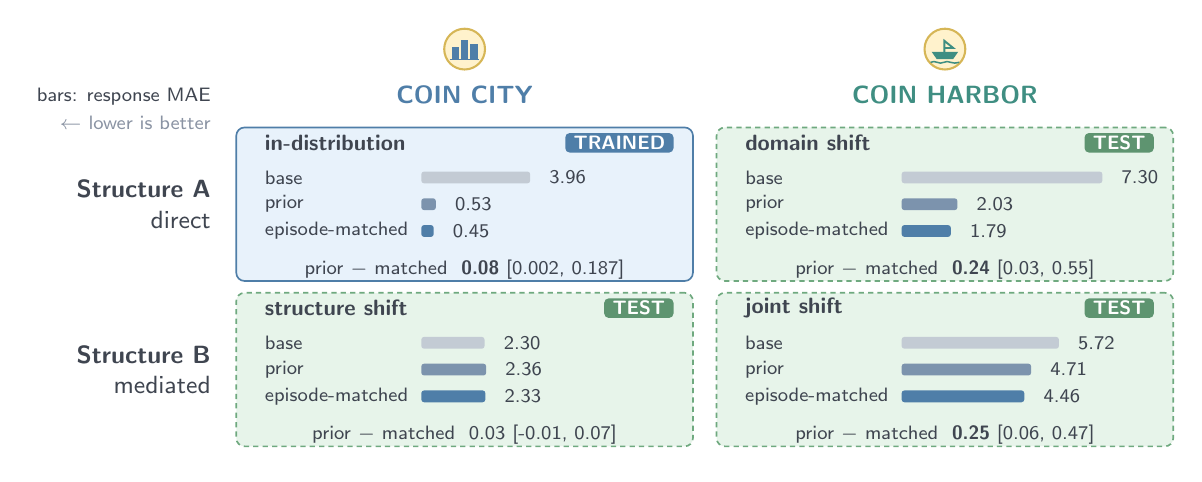
\begin{tikzpicture}[
  x=1cm, y=1cm,
  card/.style={rounded corners=3pt, minimum width=5.80cm, minimum height=1.95cm,
    line width=.6pt, inner sep=0pt},
  traincard/.style={card, draw=gCityEdge, fill=gCityFill},
  testcard/.style={card, draw=gTestEdge, fill=gTestFill,
    dash pattern=on 1.9pt off 1.5pt},
  dname/.style={anchor=south, font=\sffamily\bfseries\small},
  rname/.style={anchor=east, align=right, font=\sffamily\small, text=gInk},
  cellname/.style={anchor=west, font=\sffamily\bfseries\footnotesize, text=gInk},
  chip/.style={anchor=east, rounded corners=1.6pt, draw=none, text=white,
    inner xsep=3pt, inner ysep=1.1pt, font=\sffamily\bfseries\scriptsize},
  armlab/.style={anchor=west, font=\sffamily\scriptsize, text=gInk},
  armval/.style={anchor=west, font=\sffamily\scriptsize, text=gInk},
  delta/.style={anchor=center, font=\sffamily\scriptsize, text=gInk},
  legend/.style={anchor=east, font=\sffamily\scriptsize},
]
% ---- domain columns ------------------------------------------------------
\gcoincity{2.90}{3.22}
\gcoinharbor{9.00}{3.22}
\node[dname, text=gCityEdge]   at (2.90,2.40) {COIN CITY};
\node[dname, text=gHarborEdge] at (9.00,2.40) {COIN HARBOR};

% ---- what the bars mean, and which way is good --------------------------
\node[legend, text=gInk]  at (-0.20,2.62) {bars: response MAE};
\node[legend, text=gMute] at (-0.20,2.28) {$\leftarrow$ lower is better};

% ---- mechanism rows ------------------------------------------------------
\node[rname] at (-0.20,1.25) {\textbf{Structure A}\\ direct};
\node[rname] at (-0.20,-0.85) {\textbf{Structure B}\\ mediated};

% ---- the four result cards ----------------------------------------------
\node[traincard] at (2.90,1.25) {};
\node[testcard]  at (9.00,1.25) {};
\node[testcard]  at (2.90,-0.85) {};
\node[testcard]  at (9.00,-0.85) {};

\gcard{2.90}{1.25}{in-distribution}{TRAINED}{gCityEdge}
  {\cciIDbase}{\cciIDprior}{\cciIDmatched}
\node[delta] at (2.90,0.42) {prior $-$ matched\ \ \cciIDdelta};

\gcard{9.00}{1.25}{domain shift}{TEST}{gTestChip}
  {\cciDomainbase}{\cciDomainprior}{\cciDomainmatched}
\node[delta] at (9.00,0.42) {prior $-$ matched\ \ \cciDomaindelta};

\gcard{2.90}{-0.85}{structure shift}{TEST}{gTestChip}
  {\cciStructurebase}{\cciStructureprior}{\cciStructurematched}
\node[delta] at (2.90,-1.68) {prior $-$ matched\ \ \cciStructuredelta};

\gcard{9.00}{-0.85}{joint shift}{TEST}{gTestChip}
  {\cciJointbase}{\cciJointprior}{\cciJointmatched}
\node[delta] at (9.00,-1.68) {prior $-$ matched\ \ \cciJointdelta};
\end{tikzpicture}%
}
\caption{\textbf{Qwen3-8B Coin City transfer at round 300 under five-draw
stochastic decoding.} Bars show task-averaged response MAE over four evidence
depths; trained arms average three seeds. Each cell prints the paired seed-first
prior-minus-matched contrast, bold when its 95\% interval excludes zero.}
\label{fig:exp3-transfer-results}
\end{figure}


The trained arms have identical prompts and answer-key multisets; only the
prompt--key pairing differs. The $.251$ contrast therefore isolates the benefit of
learning how each episode's evidence maps to outcomes. It is $20\%$ of the
$1.26$-point gain over base (31\% on parsed draws); shared format and
population-distribution learning account for the rest. Episode-matched relationship
use is separable, but it is not the dominant training effect.

\textbf{Pathway-description ablation.}
In the joint cell, correct, absent, and misleading hints yield matched MAE of
$4.46$, $4.57$, and $4.77$. Removing the hint raises error by $.117$
$[.010,.230]$ and reversing it by $.309$ $[.206,.411]$, showing that pathway
descriptions still affect transferred forecasts.

\subsection{Experiment 4: Historical-Market Training and Held-Out Evaluation}
\label{sec:exp4}

Experiment~4 evaluates outcome-based training on resolved events outside its
training set. The scale analysis uses 318 markets disjoint in task, event, series,
and template family from training, development, and the 1,024-market appendix
evaluation. Figure~\ref{fig:exp4-scale-results} connects Qwen3 at 1.7B, 4B,
8B, and 14B and Llama at 3B and 8B within family on a shared parameter axis; a
categorical panel gives noncomparable frontier references. Local points use
five-draw non-thinking stochastic decoding (Appendix~\ref{app:exp4}).

\begin{center}
\begin{minipage}{\linewidth}
\centering
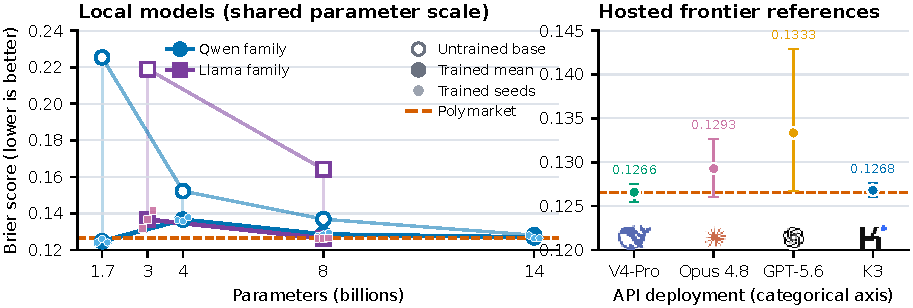
\includegraphics[width=\linewidth]{figures/exp4_qwen_scale_results.pdf}
\captionof{figure}{\textbf{Local scaling and hosted frontier references.}
Left: open/filled points are base/trained means; small points are seeds.
Right: bars are clustered 95\% intervals relative to contemporaneous Polymarket.
The panels use different axes and Brier scales.}
\label{fig:exp4-scale-results}
\end{minipage}
\end{center}

\textbf{Scale profile.}
Qwen3 trained means are $.1248$/$.1366$/$.1286$/$.1270$ at
1.7B/4B/8B/14B, versus bases $.2253$/$.1522$/$.1369$/$.1281$.
Llama trained means are $.1367$ at 3B and $.1264$ at 8B. DeepSeek and Kimi are
numerically tied with the crowd ($.12660$ and $.12682$ versus $.12655$); Anthropic
Opus~4.8 is numerically worse ($.12927$), and OpenAI GPT-5.6 is worse under
fail-closed scoring ($.13335$). API points provide context, not a scaling curve.

\textbf{Scale-comparison limits.}
At 14B, trained-minus-base is $-.00117$ $[-.00298,+.00016]$ and trained
minus the contemporaneous crowd (Brier $.12655$) is $+.00040$
$[-.00028,+.00139]$; Llama-8B minus crowd is $-.00012$
$[-.00046,+.00012]$. All three intervals cross zero. Qwen error is nonmonotone because
1.7B outperforms 4B--14B, while two Llama checkpoints cannot identify a family
curve. The results establish neither crowd superiority nor a universal scaling
law.
